\section{Monkey testing}
Monkey testing is a technique where the user tests the application by providing random inputs and checking behaviour, or seeing whether the application or system will crash.
This test has been done using \textit{Firebase Test Lab}, that is an application-testing infrastructure offered by Google Firebase.
It permits to define different device configurations' collection on which application can be tested. Every device configuration collection works on a specific range of device types, language, and orientation configuration options.
Every test is performed via virtual and physical devices located at the Google data center.
When a test is run against devices and configurations selected, \textit{Test Lab} runs the test and display the results as a \textbf{text matrix}.
\newline
\textbf{Devices x Test Executions = Test Matrix}
\begin{figure}[H]
   \centering
  \centerline{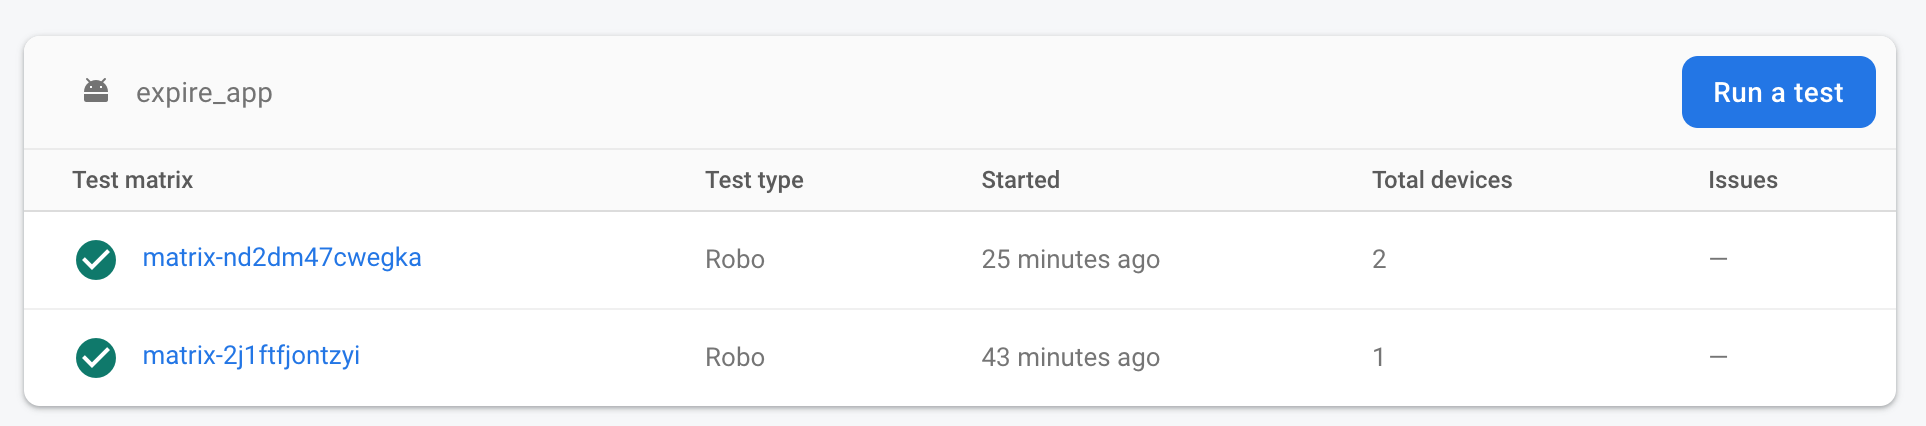
\includegraphics[width=150mm,scale=0.9]{./Images/testing/testing1.png}}
  \caption{Matrix test}
\end{figure}

Another test performed with \texit{Test Lab} is so called \textbf{robo test}.
It analyzes the structure of app's UI and explores it methodically, automatically simulating user activities.
This test captures log files, saves a series of annotated screenshots, and then creates a video form those screenshots to show the simulated operations that it performed.
\begin{figure}[H]
   \centering
  \centerline{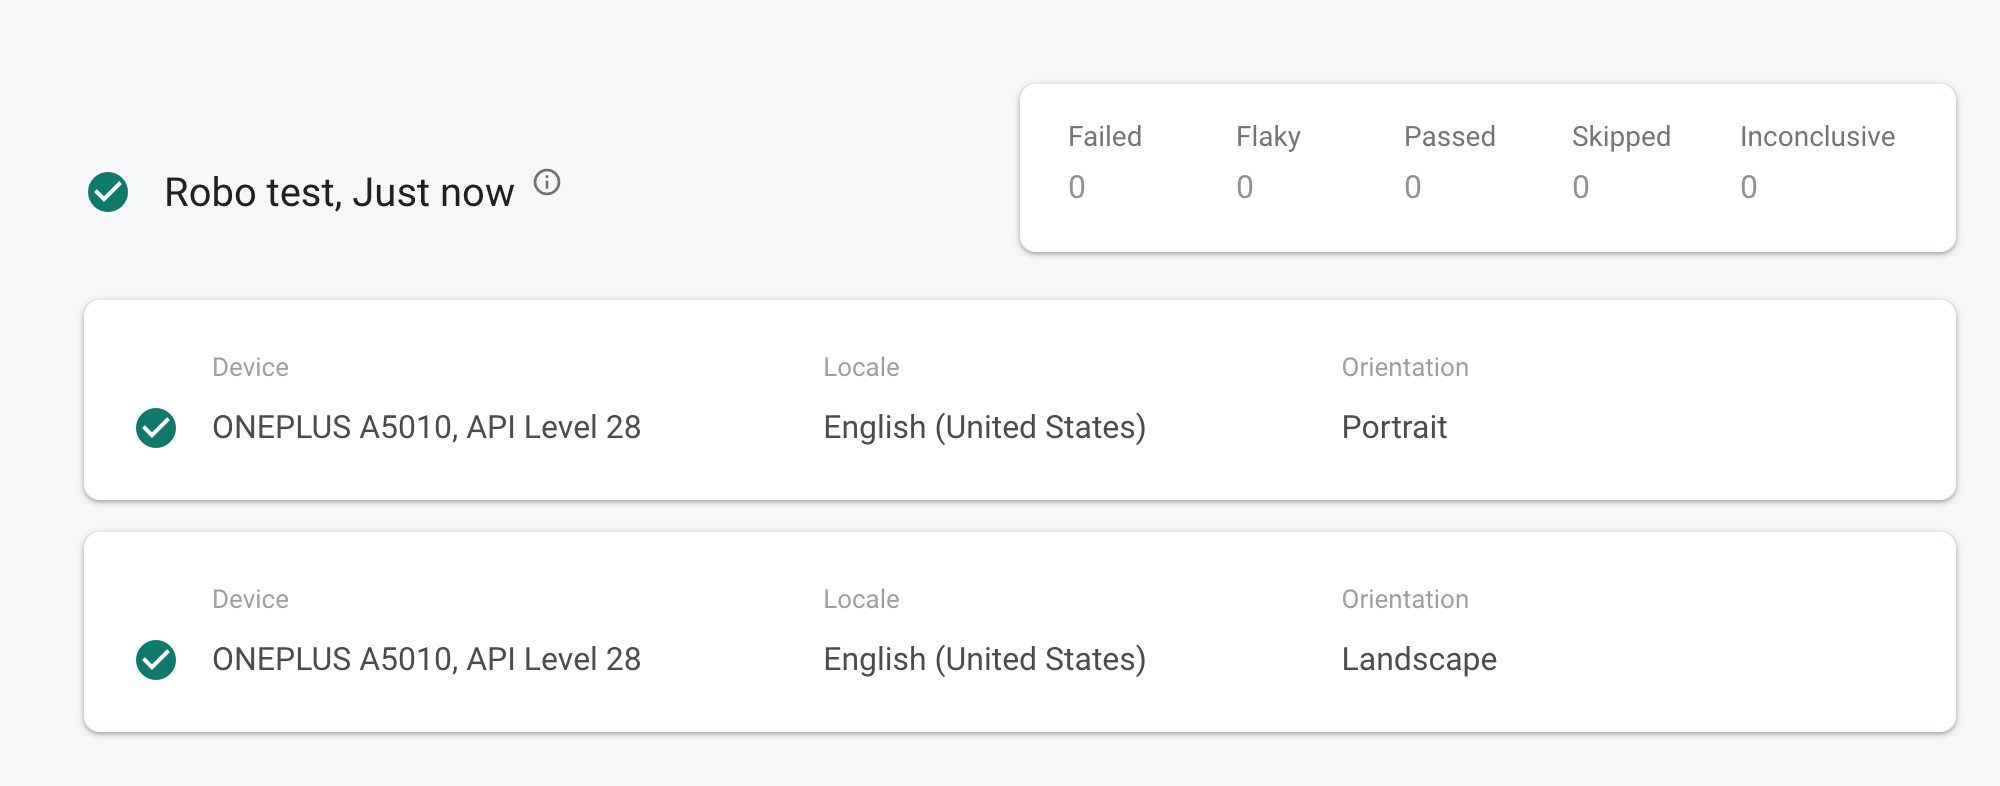
\includegraphics[width=150mm,scale=0.9]{./Images/testing/testing2.png}}
  \caption{Robo test}
\end{figure}